\documentclass[tikz, border=10pt]{standalone}
% Shared preamble — % Shared preamble — % Shared preamble — \input{preamble} in each figure file.
% Compiled via Makefile which sets TEXINPUTS so this file is always found.

% -----------------------------------------------------------------------
% Fonts — matches ntnuthesis.cls
% -----------------------------------------------------------------------
\usepackage[utf8]{inputenc}
\usepackage[T1]{fontenc}
\usepackage[charter, cal=cmcal]{mathdesign} % Charter body + math font
\usepackage[scaled=.88]{berasans}           % Bera sans-serif
\usepackage[scaled=.82]{DejaVuSansMono}     % DejaVu monospace (for \texttt)

% -----------------------------------------------------------------------
% TikZ & PGF
% -----------------------------------------------------------------------
\usepackage{tikz}
\usetikzlibrary{
  positioning,
  arrows.meta,
  fit,
  calc,
  backgrounds,
  shapes.geometric,
  shapes.multipart,
  shapes.symbols,
  shapes.callouts,
  shapes.arrows,
  shapes.misc,
  decorations.pathreplacing,
  decorations.markings,
  matrix,
}
\usepackage{pgf-umlsd}
\usepackage{pgfplots}
\usepackage{pgfplotstable}
\pgfplotsset{compat=1.18}
\usepgfplotslibrary{fillbetween}

% -----------------------------------------------------------------------
% Math
% -----------------------------------------------------------------------
\usepackage{amsmath}

% -----------------------------------------------------------------------
% Color palette
% -----------------------------------------------------------------------
% Semantic NLP / model-diagram colors
\colorlet{tok}{green!35!black}
\colorlet{emb}{yellow!70!orange}
\colorlet{trm}{blue!55!black}
\colorlet{out}{red!70!black}
% General purpose
\colorlet{clrA}{blue!60!black}
\colorlet{clrB}{orange!80!black}
\colorlet{clrC}{green!50!black}
\colorlet{clrD}{red!65!black}
\colorlet{clrE}{violet!70!black}
% Neutral fills
\colorlet{fillLight}{gray!12}
\colorlet{fillMed}{gray!25}

% -----------------------------------------------------------------------
% Global TikZ styles
% NOTE: no blank lines inside \tikzset{} — blank lines produce \par and
%       break pgfkeys parsing.
% -----------------------------------------------------------------------
\tikzset{
  >=Latex,
  % --- generic boxes ---
  box/.style={rectangle, draw, thick, align=center, inner sep=4pt, minimum height=8mm},
  rbox/.style={box, rounded corners=6pt},
  dbox/.style={box, dashed},
  % --- NLP diagram node types ---
  token/.style={rbox, draw=tok!80, fill=tok!20, minimum width=1.8cm, font=\small},
  embed/.style={box, draw=emb!90, fill=emb!30, minimum width=1.4cm},
  trm/.style={ellipse, draw=trm!90, fill=trm!20, minimum width=1.6cm, minimum height=8mm},
  output/.style={rbox, draw=out!90, fill=out!20, minimum width=1.7cm, font=\small},
  % --- arrows ---
  arrow/.style={-{Stealth[length=2mm]}, thick},
  connect/.style={->, thick, gray!65},
  darrow/.style={<->, thick},
  % --- annotation ---
  labelbox/.style={draw, thick, inner sep=4pt, rounded corners=3pt, font=\scriptsize\bfseries},
}
 in each figure file.
% Compiled via Makefile which sets TEXINPUTS so this file is always found.

% -----------------------------------------------------------------------
% Fonts — matches ntnuthesis.cls
% -----------------------------------------------------------------------
\usepackage[utf8]{inputenc}
\usepackage[T1]{fontenc}
\usepackage[charter, cal=cmcal]{mathdesign} % Charter body + math font
\usepackage[scaled=.88]{berasans}           % Bera sans-serif
\usepackage[scaled=.82]{DejaVuSansMono}     % DejaVu monospace (for \texttt)

% -----------------------------------------------------------------------
% TikZ & PGF
% -----------------------------------------------------------------------
\usepackage{tikz}
\usetikzlibrary{
  positioning,
  arrows.meta,
  fit,
  calc,
  backgrounds,
  shapes.geometric,
  shapes.multipart,
  shapes.symbols,
  shapes.callouts,
  shapes.arrows,
  shapes.misc,
  decorations.pathreplacing,
  decorations.markings,
  matrix,
}
\usepackage{pgf-umlsd}
\usepackage{pgfplots}
\usepackage{pgfplotstable}
\pgfplotsset{compat=1.18}
\usepgfplotslibrary{fillbetween}

% -----------------------------------------------------------------------
% Math
% -----------------------------------------------------------------------
\usepackage{amsmath}

% -----------------------------------------------------------------------
% Color palette
% -----------------------------------------------------------------------
% Semantic NLP / model-diagram colors
\colorlet{tok}{green!35!black}
\colorlet{emb}{yellow!70!orange}
\colorlet{trm}{blue!55!black}
\colorlet{out}{red!70!black}
% General purpose
\colorlet{clrA}{blue!60!black}
\colorlet{clrB}{orange!80!black}
\colorlet{clrC}{green!50!black}
\colorlet{clrD}{red!65!black}
\colorlet{clrE}{violet!70!black}
% Neutral fills
\colorlet{fillLight}{gray!12}
\colorlet{fillMed}{gray!25}

% -----------------------------------------------------------------------
% Global TikZ styles
% NOTE: no blank lines inside \tikzset{} — blank lines produce \par and
%       break pgfkeys parsing.
% -----------------------------------------------------------------------
\tikzset{
  >=Latex,
  % --- generic boxes ---
  box/.style={rectangle, draw, thick, align=center, inner sep=4pt, minimum height=8mm},
  rbox/.style={box, rounded corners=6pt},
  dbox/.style={box, dashed},
  % --- NLP diagram node types ---
  token/.style={rbox, draw=tok!80, fill=tok!20, minimum width=1.8cm, font=\small},
  embed/.style={box, draw=emb!90, fill=emb!30, minimum width=1.4cm},
  trm/.style={ellipse, draw=trm!90, fill=trm!20, minimum width=1.6cm, minimum height=8mm},
  output/.style={rbox, draw=out!90, fill=out!20, minimum width=1.7cm, font=\small},
  % --- arrows ---
  arrow/.style={-{Stealth[length=2mm]}, thick},
  connect/.style={->, thick, gray!65},
  darrow/.style={<->, thick},
  % --- annotation ---
  labelbox/.style={draw, thick, inner sep=4pt, rounded corners=3pt, font=\scriptsize\bfseries},
}
 in each figure file.
% Compiled via Makefile which sets TEXINPUTS so this file is always found.

% -----------------------------------------------------------------------
% Fonts — matches ntnuthesis.cls
% -----------------------------------------------------------------------
\usepackage[utf8]{inputenc}
\usepackage[T1]{fontenc}
\usepackage[charter, cal=cmcal]{mathdesign} % Charter body + math font
\usepackage[scaled=.88]{berasans}           % Bera sans-serif
\usepackage[scaled=.82]{DejaVuSansMono}     % DejaVu monospace (for \texttt)

% -----------------------------------------------------------------------
% TikZ & PGF
% -----------------------------------------------------------------------
\usepackage{tikz}
\usetikzlibrary{
  positioning,
  arrows.meta,
  fit,
  calc,
  backgrounds,
  shapes.geometric,
  shapes.multipart,
  shapes.symbols,
  shapes.callouts,
  shapes.arrows,
  shapes.misc,
  decorations.pathreplacing,
  decorations.markings,
  matrix,
}
\usepackage{pgf-umlsd}
\usepackage{pgfplots}
\usepackage{pgfplotstable}
\pgfplotsset{compat=1.18}
\usepgfplotslibrary{fillbetween}

% -----------------------------------------------------------------------
% Math
% -----------------------------------------------------------------------
\usepackage{amsmath}

% -----------------------------------------------------------------------
% Color palette
% -----------------------------------------------------------------------
% Semantic NLP / model-diagram colors
\colorlet{tok}{green!35!black}
\colorlet{emb}{yellow!70!orange}
\colorlet{trm}{blue!55!black}
\colorlet{out}{red!70!black}
% General purpose
\colorlet{clrA}{blue!60!black}
\colorlet{clrB}{orange!80!black}
\colorlet{clrC}{green!50!black}
\colorlet{clrD}{red!65!black}
\colorlet{clrE}{violet!70!black}
% Neutral fills
\colorlet{fillLight}{gray!12}
\colorlet{fillMed}{gray!25}

% -----------------------------------------------------------------------
% Global TikZ styles
% NOTE: no blank lines inside \tikzset{} — blank lines produce \par and
%       break pgfkeys parsing.
% -----------------------------------------------------------------------
\tikzset{
  >=Latex,
  % --- generic boxes ---
  box/.style={rectangle, draw, thick, align=center, inner sep=4pt, minimum height=8mm},
  rbox/.style={box, rounded corners=6pt},
  dbox/.style={box, dashed},
  % --- NLP diagram node types ---
  token/.style={rbox, draw=tok!80, fill=tok!20, minimum width=1.8cm, font=\small},
  embed/.style={box, draw=emb!90, fill=emb!30, minimum width=1.4cm},
  trm/.style={ellipse, draw=trm!90, fill=trm!20, minimum width=1.6cm, minimum height=8mm},
  output/.style={rbox, draw=out!90, fill=out!20, minimum width=1.7cm, font=\small},
  % --- arrows ---
  arrow/.style={-{Stealth[length=2mm]}, thick},
  connect/.style={->, thick, gray!65},
  darrow/.style={<->, thick},
  % --- annotation ---
  labelbox/.style={draw, thick, inner sep=4pt, rounded corners=3pt, font=\scriptsize\bfseries},
}


% -----------------------------------------------------------------------
% Local styles (extend preamble's rbox / connect)
% -----------------------------------------------------------------------
\tikzset{
    container/.style={
        draw=#1!70,
        fill=#1!8,
        rounded corners=6pt,
        thick,
        align=center,
        rectangle split,
        rectangle split parts=2,
        inner sep=6pt,
        font=\small,
        text width=3.6cm,
        rectangle split part fill={#1!25, #1!8},
        rectangle split part align={center, center},
    }
}

\begin{document}
    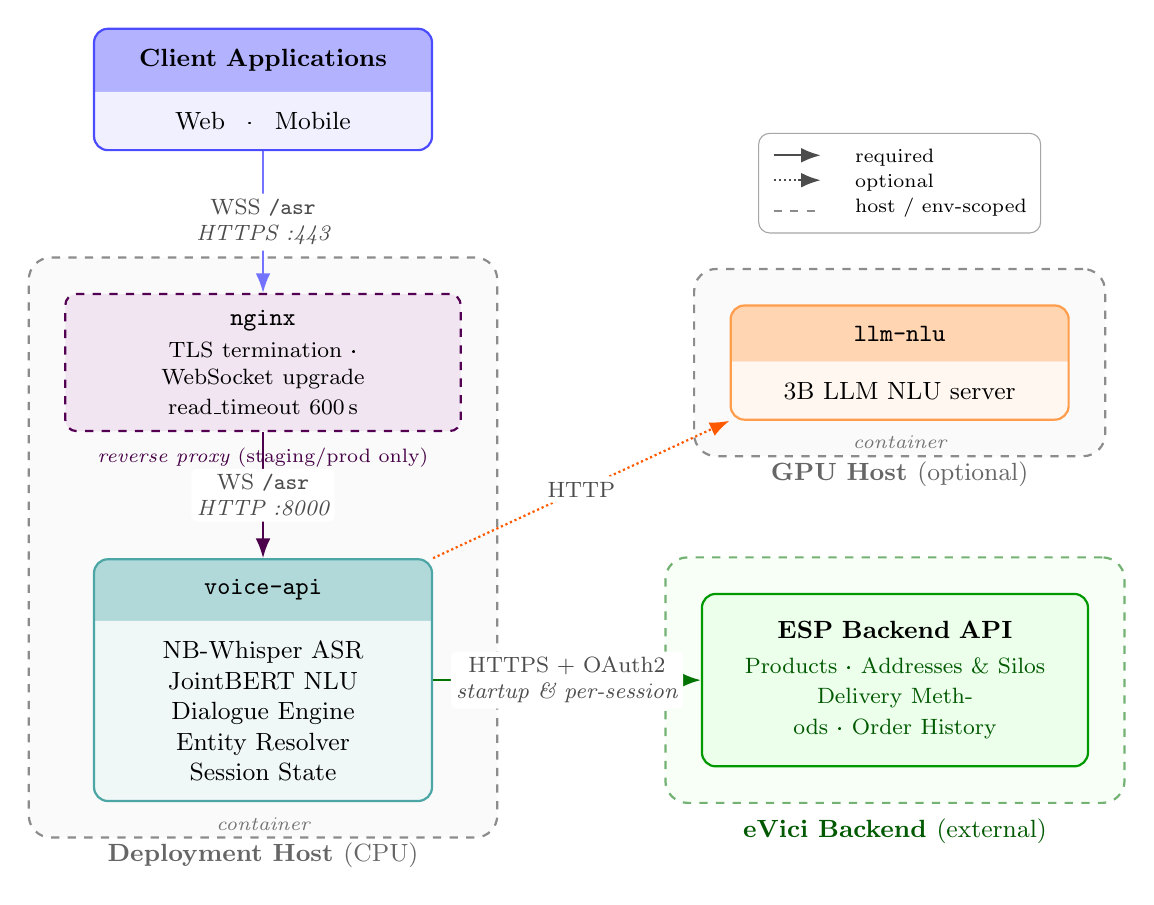
\begin{tikzpicture}[
        font=\small,
        node distance=1.8cm and 2.0cm,
        flow/.style     = {-{Latex[length=2.5mm]}, thick, #1},
        flow/.default   = black!70,
        optional/.style = {-{Latex[length=2.5mm]}, thick, densely dotted, #1},
        optional/.default = black!55,
        edgelabel/.style = {font=\footnotesize, text=black!70,
                            fill=white, inner sep=2pt, rounded corners=2pt},
        component/.style n args={2}{
            draw=#1!70, thick, rounded corners=5pt,
            rectangle split, rectangle split parts=2,
            rectangle split part fill={#1!30, #1!6},
            rectangle split draw splits=false,
            inner sep=7pt, align=center,
            text width=3.8cm, font=\small,
            label={[font=\scriptsize\itshape, text=black!55,
                    yshift=-2pt]below:#2}
        },
        proxy/.style={
            draw=violet!65!black, thick, dashed, rounded corners=4pt,
            fill=violet!10, align=center, inner sep=6pt,
            text width=4.6cm, font=\small,
            label={[font=\scriptsize\itshape, text=violet!55!black,
                    yshift=-2pt]below:reverse proxy \normalfont(staging/prod only)}
        },
        external/.style={
            draw=#1!60!black, fill=#1!8, rounded corners=5pt, thick,
            align=center, inner sep=10pt, text width=4.2cm, font=\small,
        },
        badge/.style={
            draw=orange!70!red, fill=orange!20,
            rounded corners=3pt, inner sep=2pt,
            font=\scriptsize\bfseries, text=orange!55!red,
        },
        host/.style={
            draw=black!45, dashed, rounded corners=8pt,
            fill=black!2, thick, inner sep=0.45cm,
        },
    ]

    %% ── Client ───────────────────────────────────────────────
    \node[component={blue}{}] (client) {
        \textbf{Client Applications}
        \nodepart{two}
        Web \enspace · \enspace Mobile
    };

    %% ── nginx reverse proxy (inside CPU host) ────────────────
    \node[proxy, below=1.8cm of client] (nginx) {
        \textbf{\ttfamily nginx} \\[2pt]
        {\footnotesize TLS termination · WebSocket upgrade \\
         read\_timeout 600\,s}
    };

    %% ── voice-api (CPU) ──────────────────────────────────────
    \node[component={teal}{container}, below=1.6cm of nginx] (voice) {
        \textbf{\ttfamily voice-api}
        \nodepart{two}
        NB-Whisper ASR \\
        JointBERT NLU \\
        Dialogue Engine \\
        Entity Resolver \\
        Session State
    };

    %% ── llm-nlu (GPU) — now up next to nginx ─────────────────
    \node[component={orange!90!red}{container}, right=3.4cm of nginx]
        (llm) {
        \textbf{\ttfamily llm-nlu}
        \nodepart{two}
        3B LLM NLU server
    };

    %% ── ESP Backend — now right of voice-api ─────────────────
    \node[external=green, right=3.4cm of voice] (esp) {
        \textbf{ESP Backend API} \\[3pt]
        {\footnotesize\color{green!35!black}
            Products · Addresses \& Silos \\
            Delivery Methods · Order History}
    };

    %% ── Boundaries ───────────────────────────────────────────
    \begin{pgfonlayer}{background}
        \node[host, fit=(nginx)(voice),
              label={[font=\small\bfseries, text=black!60,
                      yshift=2pt]below:Deployment Host \normalfont(CPU)}]
              (cpuhost) {};
        \node[host, fit=(llm),
              label={[font=\small\bfseries, text=black!60,
                      yshift=2pt]below:GPU Host \normalfont(optional)}]
              (gpuhost) {};
        \node[draw=green!45!black!55, dashed, rounded corners=8pt,
              fill=green!3, thick, inner sep=0.45cm, fit=(esp),
              label={[font=\small\bfseries, text=green!35!black,
                      yshift=-2pt]below:eVici Backend \normalfont(external)}]
              (espbound) {};
    \end{pgfonlayer}

    %% ── Arrows ───────────────────────────────────────────────
    % Client → nginx
    \draw[flow=blue!55]
        (client) -- node[edgelabel, align=center]
            {WSS \texttt{/asr} \\ \itshape HTTPS :443}
        (nginx.north);

    % nginx → voice-api
    \draw[flow=violet!60!black]
        (nginx.south) -- node[edgelabel, align=center]
            {WS \texttt{/asr} \\ \itshape HTTP :8000 }
        (voice.north);

    % voice-api → llm-nlu (optional, diagonal up-right)
    \draw[optional=orange!70!red]
        (voice.north east) -- node[edgelabel, align=center, pos=0.5]
            {HTTP}
        (llm.south west);

    % voice-api → ESP (horizontal right)
    \draw[flow=green!45!black]
        (voice.east) -- node[edgelabel, align=center]
            {HTTPS + OAuth2 \\ \itshape startup \& per-session}
        (esp.west);

    %% ── Legend (below ESP, compact) ──────────────────────────
    \node[draw=black!35, rounded corners=4pt, fill=white,
          inner sep=5pt, font=\scriptsize,
          above=0.9cm of llm] (legend) {
        \begin{tabular}{@{}ll@{}}
            \tikz\draw[flow=black!70] (0,0)--(0.6,0); & required \\[1pt]
            \tikz\draw[optional=black!70] (0,0)--(0.6,0); & optional \\[1pt]
            \tikz\draw[dashed, thick, black!45] (0,0)--(0.6,0); & host / env-scoped \\
        \end{tabular}
    };
    \end{tikzpicture}
\end{document}
